\documentclass[12pt]{article}

\usepackage{multicol}
\usepackage{sbc-template}
\usepackage{graphicx,url}
\usepackage[utf8]{inputenc}
\usepackage[brazil]{babel}

\usepackage{longtable}
\usepackage{changepage}
     
\sloppy

\title{Modelagem contextualizada da movimentação de jogadores em uma partida de futebol}
\author{Lucca Augusto\inst{1}}
\address{Universidade Federal de Minas Gerais (UFMG)\\
  \email{luccaaugusto@gmail.com}
}
\begin{document}
\maketitle

% \begin{resumo} \end{resumo}

\section{Introdução}\label{int}
O avanço em modelos de Inteligência Artificial (IA) vem revolucionando as mais diversas áreas, como a predição da estrutura de proteínas \cite{alphafold}, criação de imagens a partir de texto \cite{dalle} e até IAs de propósito geral como o Chat-GPT \cite{chatgpt}. Com o esporte não é diferente, técnicas de IA vêm auxiliando os profissionais da área em todas as fases, como na captação de potenciais bons esportistas, no treino, durante o jogo e na análise pós-jogo. \looseness=-1

Uma tarefa muito pesquisada é análise de possíveis diferentes cenários, popularmente conhecidos como \textit{``What if ..."}, ou traduzindo ``E se...", como por exemplo na questão: ``E se fôssemos iguais? Uma comparação entre a diferença de mortalidade entre brancos e negros" \cite{satcher2005if}. Nos esportes isso normalmente acontece quando queremos prever como uma jogada aconteceria caso um ou mais jogadores tomassem decisões diferentes, e já há algumas iniciativas utilizando IA em perguntas do tipo. \looseness=-1

Um dos grandes desafios nos esportes é prever ou sintetizar a movimentação, o que é de uma enorme importância para análises \textit{what-if} da maioria das jogadas. Em \cite{le2017data}, o objetivo é prever o melhor posicionamento dos jogadores em determinada situação ou até como diferentes times agiriam, enquanto em \cite{graphcounteratack} a ideia principal é sugerir pequenas correções para aumentar a efetividade de um contra-ataque, como a direção de deslocamento de um jogador. \looseness=-1

Ambos estudos tem uma limitação, que é ignorar a movimentação corretiva do time oposto dado à mudança de posicionamento sugerida pelo modelo, ou seja, a sugestão de melhoria só é válida caso o time adversário permaneça imóvel, o que é claramente irreal. Com isso surge a necessidade de maiores estudos na predição e geração da movimentação de todos os jogadores, ou seja, considerando os dois times. \looseness=-1

Dada a diversidade de cenários no futebol, propomos delimitar o escopo dos modelos a serem investigados para tipos de jogada específicos, evitando cenários demasiadamente genéricos, tal qual \cite{graphcounteratack}, que foca apenas em contra-ataques. No nosso caso, propomos inicialmente como cenário a saída de bola, ou seja, qualquer jogada de bola parada (falta, tiro de meta ou lateral) que acontecer no terço inicial do campo. \looseness=-1

O objetivo final é desenvolver um modelo de geração da movimentação dos jogadores para saídas de bola e combiná-lo com modelos já existentes na literatura para encontrar a melhor jogada, como \cite{power2017not}, criando um modelo que sugira as melhores jogadas dentro de uma janela temporal (Figura~\ref{fig:modelo-completo}), e não só no momento inicial. Uma questão exemplo aqui é ``E se eu tocar para o jogador X, será melhor do que tocar para o jogador Y?". Nesse caso, ao invés de apenas recomendar que a melhor decisão seria passar a bola para o jogador X, pode-se mostrar que, passando para o jogador X, ele não teria boas opções para a continuidade do lance, devido à movimentação estimada, e então seria melhor passar para o jogador Y, mesmo que a princípio parecesse pior que tocar para o jogador X, uma vez que posteriormente ele consegue acionar o jogador X em uma situação melhor. \looseness=-1

\begin{figure}
    \centering
    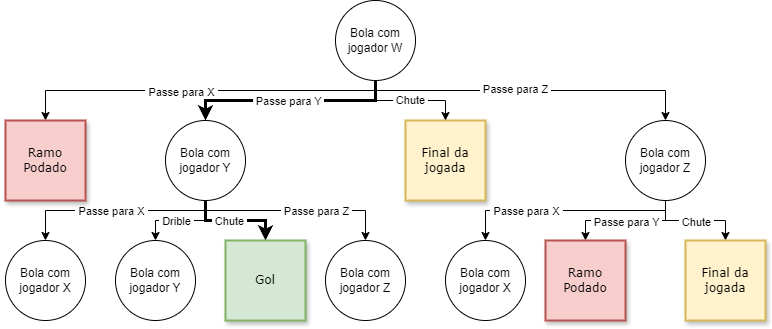
\includegraphics[scale=0.4]{images/Modelo Completo.png}
    \caption{Exemplo de uma árvore de decisões que o modelo percorrerá}
    \label{fig:modelo-completo}
\end{figure}

A principal contribuição esperada deste trabalho é a criação do modelo para gerar a movimentação de todos os jogadores a partir de um \textit{frame} dos dados de \textit{tracking} em uma saída de bola em uma partida de futebol, de forma que ele possa ser utilizado em qualquer situação de saída de bola, seja um modelo de recomendação da melhor movimentação para seus zagueiros, da melhor formação para cobrança de tiro de meta ou como os atacantes devem pressionar no caso do time com a posse tentar sair com passes curtos. O modelo final é, principalmente, um exemplo de uso aplicado para o modelo de movimentação.  \looseness=-1

Para avaliação do modelo de movimentação dos jogadores, a forma ideal seria a validação de profissionais da área de que as jogadas recomendadas não são distinguíveis das jogadas existentes, tal qual foi aplicado em \cite{tacticai} com os profissionais do Liverpool. Já para o modelo de sugestão de jogadas, podem ser utilizadas métricas amplamente conhecidas, como a soma ou média do \textit{Expected Threat} (xT) gerado em toda a jogada ou métricas personalizadas, \textit{e.g.:} quantia de metros que a bola avançou em direção ao gol desde o início da jogada. \looseness=-1

\section{Referencial Teórico}\label{ref}

Em vários esportes, a análise de dados já é algo muito consolidado e uma das histórias mais famosas, contada no livro Moneyball~\cite{moneyball}, que mais tarde virou filme, mostra como um time de beisebol foi formado apenas com dados estatísticos. A IA vem para potencializar isso, auxiliando analistas a terem novas e diferentes percepções, como em \cite{reviewbasketball}, onde o estudo é focado em revisar análises de arremessos no basquete baseadas em IA. \looseness=-1

Quando vamos para a área de movimentação no futebol, temos estudos desde métricas para avaliar pressão~\cite{pressing}, que analistas podem utilizar para ver o progresso do time neste fundamento, até preditores de movimentação de um determinado time em uma jogada~\cite{le2017data}, modelo de extrema valia para estimar como seu próximo adversário se comportaria num ataque do seu time, por exemplo. \looseness=-1

A avaliação de modelos geradores de dado sintético é um tanto quanto complexa, a depender do cenário, e no cenário da movimentação feita por seres humanos metrificar isso não é trivial. Em \cite{tacticai} uma forma de avaliação não muito comum no meio do futebol é introduzida, a opinião de especialistas, e apesar do cenário diferente da movimentação, um dos objetivos do trabalho é gerar jogadas de escanteio sintéticas, o que se assemelha bastante ao formato do modelo aqui proposto. \looseness=-1

\section{Metodologia}\label{met}
Este projeto tem uma metodologia teórica-experimental, a qual abrange o estudo da literatura sobre movimentação de jogadores, parte mais complexa e crucial do trabalho, e sobre sugestão de jogadas. Além do estudo, há a etapa de desenvolvimento dos modelos e métricas propostos. A metodologia é ilustrada pela Figura~\ref{fig:fluxograma-metodologia} e é descrita a seguir: \looseness=-1
\begin{figure}
    \centering
    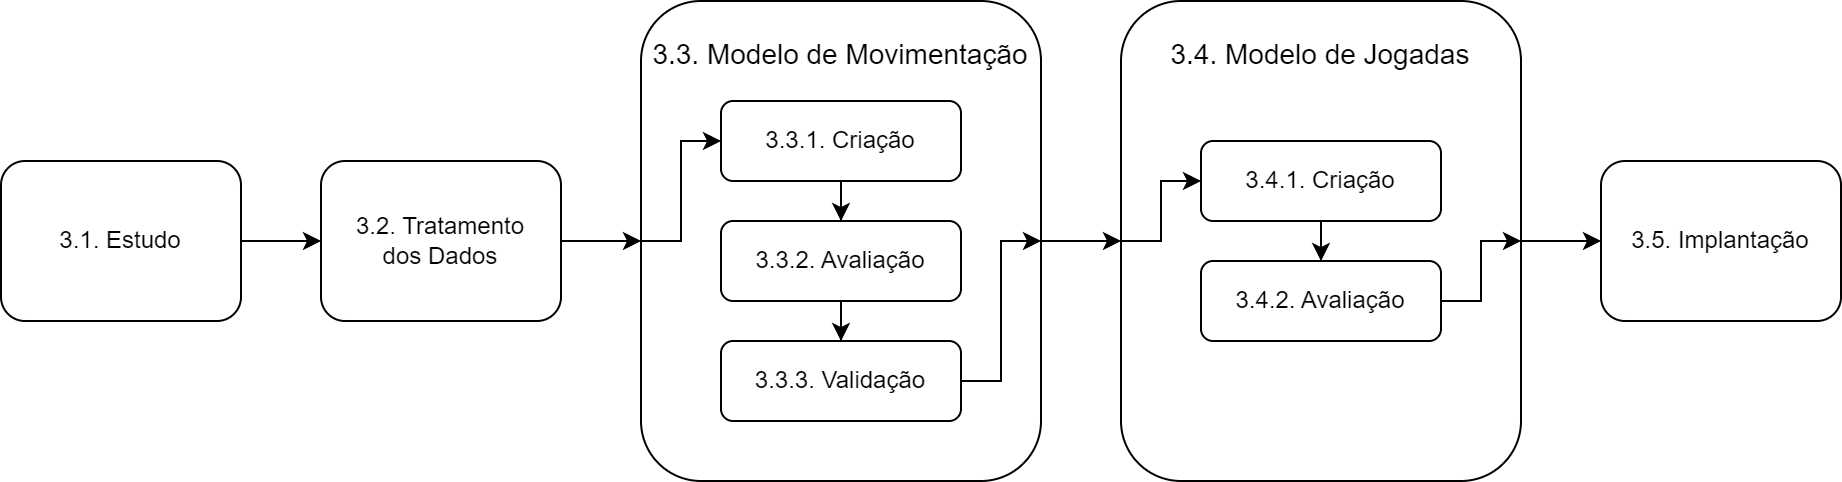
\includegraphics[scale=0.2]{images/Metodologia no Mestrado.png}
    \caption{Fluxograma da Metodologia}
    \label{fig:fluxograma-metodologia}
\end{figure}

\subsection{Estudo}\label{est}
Esta primeira parte consiste na melhor compreensão dos dados e conhecimentos necessários para a geração de movimentação dos jogadores, desde a parte física (como velocidade máxima e aceleração de arrancada) até a parte computacional (como modelagem das possibilidades de movimentação e heurísticas para poda das movimentações ruins). \looseness=-1

\subsection{Tratamento dos Dados}\label{dad}
Por meio de uma parceria do Laboratório de \textit{Sports Analytics} (SALab) da Universidade Federal de Minas Gerais (UFMG) com a PFF, uma fornecedora de dados do mundo esportivo, temos acesso aos dados necessários para a pesquisa, que são os dados de \textit{tracking} de algumas das maiores ligas do mundo, como o Basileirão (Brasil) e a \textit{Premier League} (Inglaterra). Com os dados em mãos, é necessário selecionar apenas aqueles que iniciam a jogada no terço inicial, e então fazer a limpeza e o tratamento para uso no modelo. \looseness=-1

\subsection{Modelo de Geração da Movimentação de Jogadores (MOV)}\label{mov}
A geração da movimentação dos jogadores é o modelo principal e de maior contribuição para a literatura, a construção de tal modelo será dividida em três partes, descritas a seguir: \looseness=-1

\subsubsection{Criação}\label{mov:cri}
A criação do modelo consiste na seleção de \textit{features} (características) a serem usadas, implementação da modelagem do movimento, criação e implementação da IA.\looseness=-1

\subsubsection{Avaliação}\label{mov:aval}
A sub-etapa de avaliação consiste na criação de uma métrica que permita, inicialmente, avaliar minimamente a qualidade do modelo criado, de forma que possa auxiliar no processo de desenvolvimento do modelo, como uma função de \textit{loss} (perda) específica. \looseness=-1

\subsubsection{Validação}\label{mov:val}
Trazer a opinião de especialistas é sempre interessante, mas nesse caso é imprescindível, pois não existe movimentação certa ou errada, e o que temos são movimentações que fazem sentido ou não. A validação portanto é feita em um teste não supervisionado com os especialistas, mostrando lances reais e sintéticos gerados pelo modelo: a cada jogada apresentada o especialista deve indicar se é real ou sintética, e com isso temos uma forma de quantificar, comparando acertos e erros. \looseness=-1

\subsection{Modelo de Sugestão de Jogadas (JOG)}\label{jog}
Partindo do modelo anterior, cuja as movimentações por pressuposto são naturais e próximas às reais, podemos criar um modelo que sequencialmente sugira boas jogadas, combinando o modelo desenvolvido com aqueles que fazem uma tomada de decisão. Os processos dessa etapa são descritos a seguir: \looseness=-1

\subsubsection{Criação}\label{jog:cri}
A criação do modelo consiste na escolha do modelo de tomada de decisão a ser usado, adaptação dos dados (como novas \textit{features}) gerados pelo modelo de geração de jogadores (especificado no Capítulo~\ref{mov}), definição do que será o fim de uma jogada e finalmente a integração do modelo. \looseness=-1

\subsubsection{Avaliação}\label{jog:aval}
A medida avaliativa aqui deve ser definida a partir de um estudo mais aprofundado, o que impactará e será impactado também pelo final da jogada escolhido na fase de criação (Capítulo~\ref{jog:cri}). As ideias iniciais são: agregação de métricas já existentes, como xT ou VAEP; pontuações discretas relacionadas à distância que a bola evoluiu dentro de uma janela temporal; ou a criação de outra métrica mais complexa com foco maior neste problema. \looseness=-1

\subsection{Implantação}\label{imp}
Com o código de ambos modelos pronto e validado, a ideia é disponibilizá-los para uso geral, por meio da biblioteca \textit{gandula}~\footnote{https://github.com/SALabUFMG/gandula}, uma biblioteca em \textit{python} desenvolvida pelo SALab com foco em ciência de dados no mundo do futebol. \looseness=-1


\section{Cronograma}\label{cron} \looseness=-1

Esta seção visa mostrar o cronograma planejado do projeto e das disciplinas a cursar. \looseness=-1

\begin{multicols}{2} \looseness=-1

\subsection{Projeto}\label{cron:proj} \looseness=-1

\begin{center}
\begin{tabular}{ | c | l | }
\hline
 \multicolumn{1}{| c |}{\textbf{Período}} & \multicolumn{1}{| c |}{\textbf{Atividade}} \\ \hline
 08/24 - 11/24 & Estudo \\ \hline
 11/24 - 12/24 & Tratamento dos Dados \\ \hline
 01/25 - 12/25 & MOV - Criação \\ \hline
 08/25 - 10/25 & MOV - Avaliação \\ \hline
 10/25 - 12/25 & MOV - Validação \\ \hline
 01/26 - 06/26 & JOG - Criação \\ \hline
 04/26 - 05/26 & JOG - Avaliação \\ \hline
 05/26 - 06/26 & Implantação \\ \hline
\end{tabular}
\end{center} \looseness=-1


\subsection{Disciplinas}\label{cron:disc} \looseness=-1

\begin{center}
\begin{tabular}{ | c | l | }
\hline
 \multicolumn{1}{| c |}{\textbf{Semestre}} & \multicolumn{1}{| c |}{\textbf{Matéria}} \\ \hline
 24/1 & Aprendizado Descritivo \\ \hline
 24/2 & Projeto e Análise de Algoritmos \\ \hline
 24/2 & Teoria dos Grafos \\ \hline
 25/1 & Otimização Combinatória \\ \hline
 25/2 & Inteligência Artificial \\ \hline
 26/1 & Estágio em docência \\ \hline
\end{tabular}
\end{center} \looseness=-1

\end{multicols} \looseness=-1

\bibliographystyle{sbc}
\bibliography{sbc-template}

\end{document}
